\chapter{Evaluation}
This project was meant to test the responses of such an open-source Intrusion Detection and Prevention System (IDPS) as Suricata to the simulated UDP flood attack with the help of the GNS3 emulator. During the experiment, a series of testing scenarios were introduced to have a glimpse of the performance of Suricata in different intensities of network based attacks. The contents were a baseline simulation of UDP flood attack with no detection or prevention, the second scenario in which Suricata was deployed in IPS mode and used NFQUEUE to capture malicious packets and drop them, and the third simulation in which UDP traffic was limited in rate to employ reduced volume of attacks to assess the functionality of Suricata.
\\
The experimental findings affirmed that Suricata was capable of detecting and rejecting a considerable amount of malicious UDP packets, in particular, in the case when the flood rate was moderate. By monitoring in real-time using Wireshark and logging traffic with Suricata using fast.log and eve.json, it was clear that the IPS mechanism was able to work as anticipated, that is, it could trigger alerts and set drop verdicts on traffic patterns that tend to be unusual behaving based on custom detection rules.
\\
However, the limitations arise during the simulations of the attacks of massive volume. The Suricata only dropped a part of the traffic in the flood of 40,000 packets within a brevity hence allowing a reasonable number of packets to proceed to the target system. The latter is ascribed to the host-based IPS inherent weaknesses, which tend to be restricted by CPU power, queue management and kernel capability to run a high-forwarding packet rates. Notwithstanding these shortcomings, the test proved that Suricata can be considered a good defense means particularly when used as a component of the multiple security strategy. The logs, the accuracy of matching the rules and the packet drop behavior all indicate the potential of Suricata as an active defense instrument with the proper configuration.
\pagebreak
\begin{figure}[!htb]
    \centering
    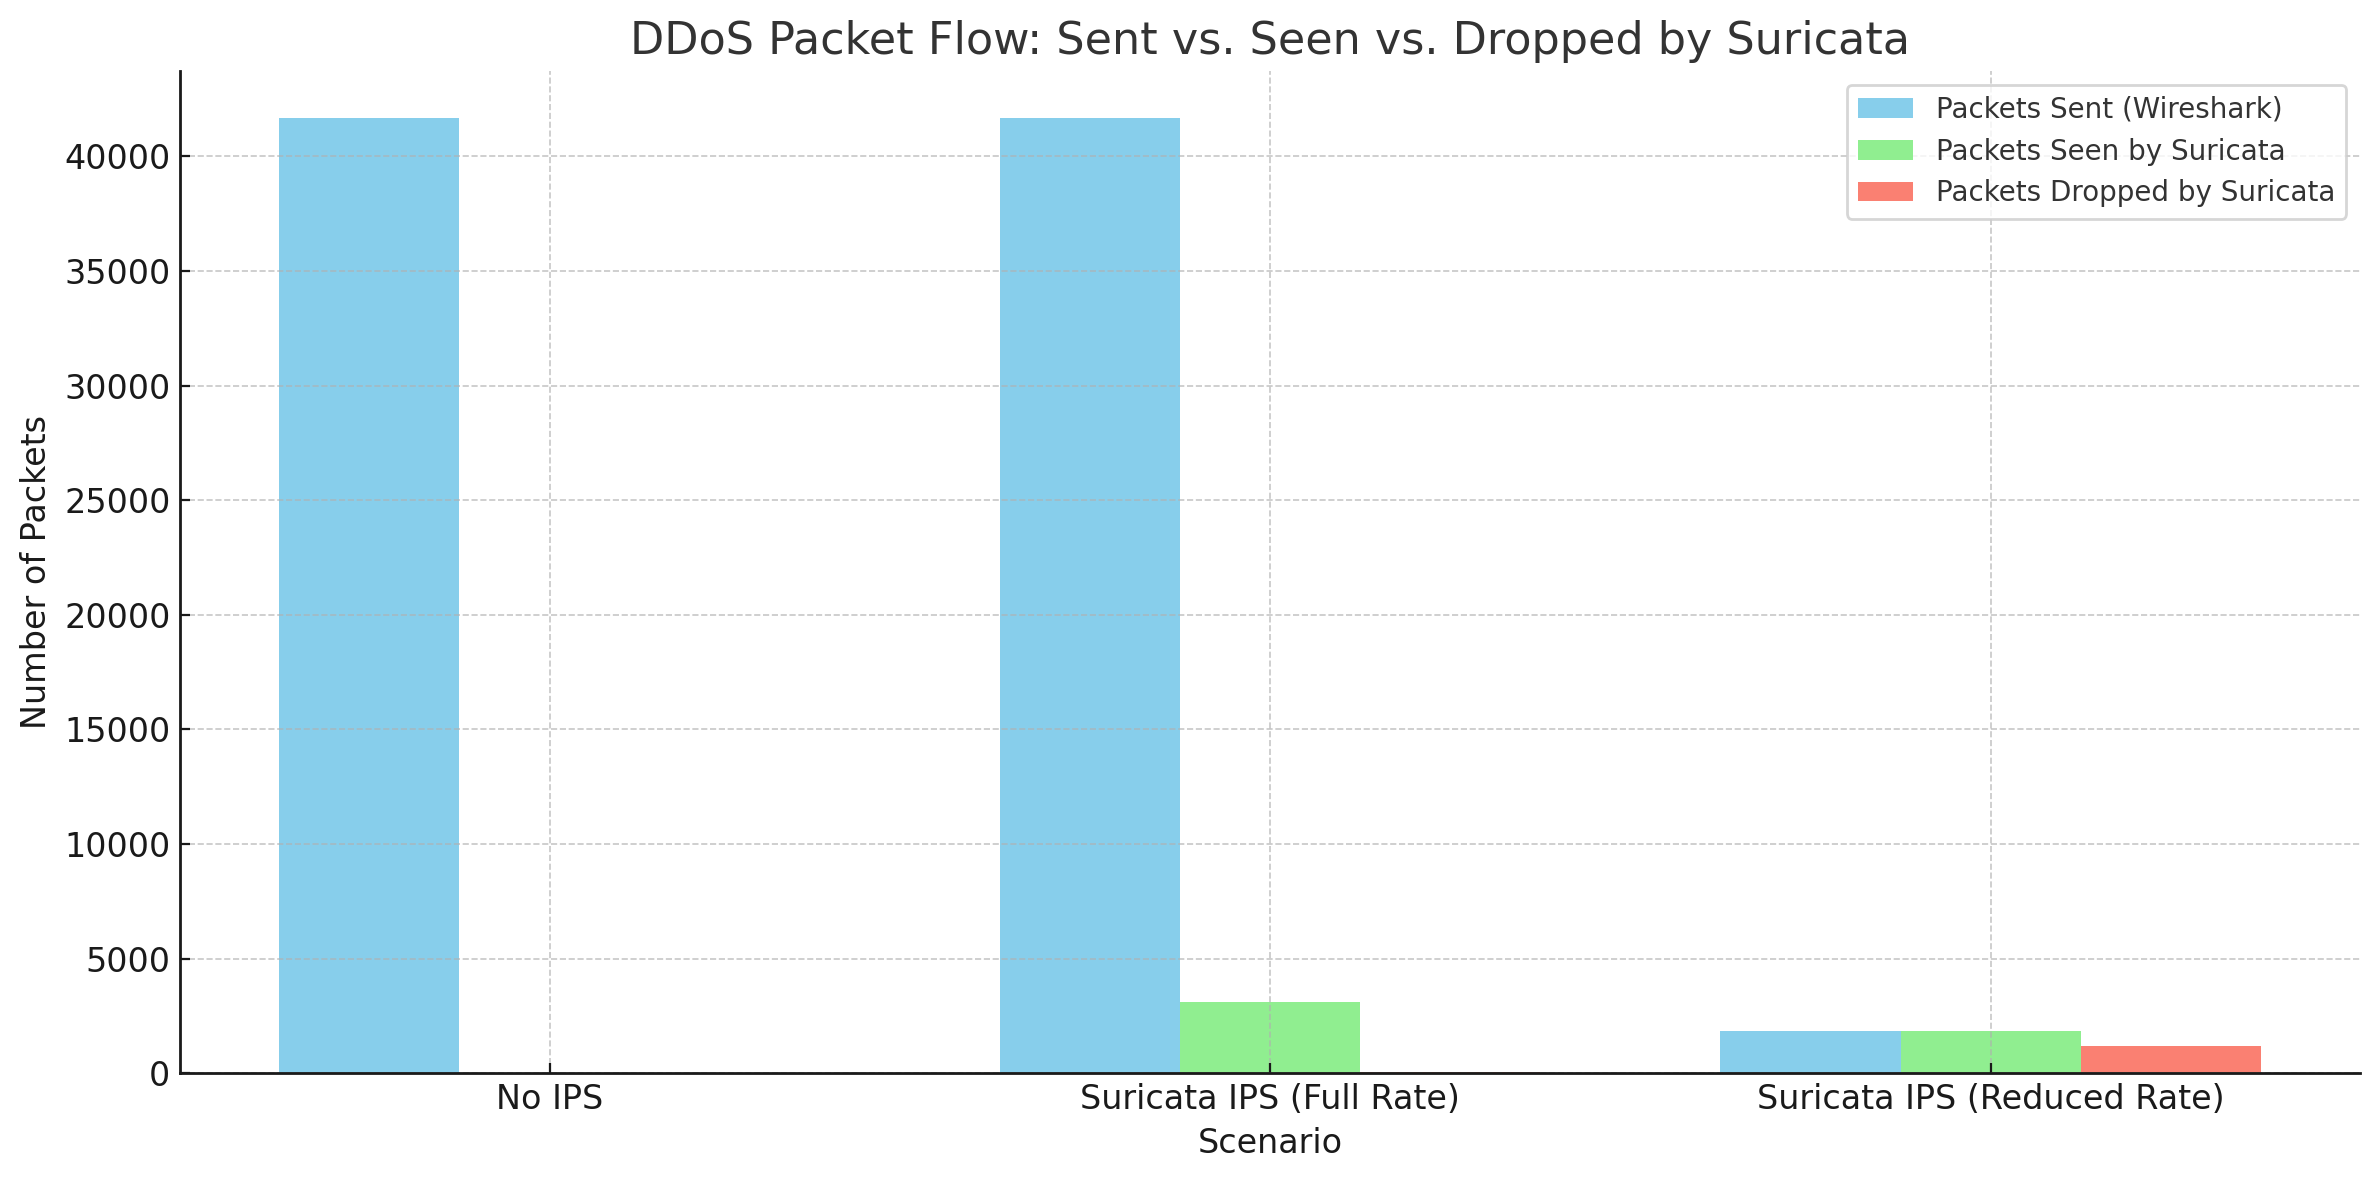
\includegraphics[scale=0.2]{thesis/evaluation.png}
    \caption{Traffic of 3 scenarios chart}
    \label{fig:enter-label}
\end{figure}
